\documentclass[11pt, a4paper]{article} 
\usepackage[utf8]{inputenc}
\usepackage[nolist,nohyperlinks]{acronym}
\usepackage{geometry}
\usepackage{setspace}

\usepackage{biblatex}
\usepackage[hidelinks]{hyperref}
\usepackage{nameref}

\usepackage{graphicx}
\usepackage{float}
\usepackage[hypcap=false]{caption}
\usepackage{subcaption}

\usepackage{tabularx}
\usepackage{multirow}

\usepackage{lipsum}

\usepackage{textcomp} % supress warning
\usepackage{gensymb} % added by Steffen


\onehalfspacing
\addbibresource{arfeedback.bib}

% TabularX column defintions
\newcolumntype{L}[1]{>{\raggedright\let\newline\\\arraybackslash\hspace{0pt}}m{#1}}
\newcolumntype{C}[1]{>{\centering\let\newline\\\arraybackslash\hspace{0pt}}m{#1}}
\newcolumntype{R}[1]{>{\raggedleft\let\newline\\\arraybackslash\hspace{0pt}}m{#1}}

% Original assignment: Evaluate how to react on wrong AR usage
\newcommand{\mytitle}{Evaluation of Textual Feedback for Incorrect Usage of an Augmented Reality Application}
\newcommand{\runninghead}{Feedback for Augmented Reality}
\newcommand{\myauthor}{Julian Lüken, Mehmed Mustafa, Jan Schneider,\\ Steffen Tunkel, Chris Warin}
\newcommand{\myuni}{Georg-August University, Göttingen}
\newcommand{\titlespace}{.9em}

% Header
\markright{\uppercase{\runninghead}\hfill}
\newenvironment{myabstract}{\begin{abstract}\begin{itshape}}{\end{itshape}\end{abstract}}

\begin{document}
	% Acronyms go here, refer to them with \ac{shorthand}
	\begin{acronym}
		\acro{AR}{Augmented Reality}
		\acro{SUS}{System Usability Scale}
	\end{acronym}

	\newgeometry{left=25mm,right=25mm,top=30mm,bottom=30mm}
	\pagestyle{empty}
	\begin{center}
		\begin{minipage}{.8\textwidth}
			\centering
			\begin{doublespace}\huge\textbf{\mytitle}\normalsize\\[\titlespace]\end{doublespace}
			\textsc{\myauthor}\\[\titlespace]
			\today\\[\titlespace]
			\myuni
		\end{minipage}
	\end{center}
	\vspace{0em}
	\begin{myabstract}
		% Abstract goes here
		\lipsum[1-2]
	\end{myabstract}

	% REMEMBER
	%
	% Write in active, not passive
	% Write as "we"
	% Only two tenses (present and past)
	% Use LaTeX acronym environment (use \ac{shorthand} and define them right after \begin{document})
	% No paragraphs with only one sentence
	% No different types of paragraphs for pseudo-structuring
	% No forward references
	% Cite consistently and clearly (\cite{Lastname1999}, Jabref)
	% Footnotes: Just where really required
	% No repetitions

	\section*{Introduction}\label{sec:introduction}
		% Motivation
		% * Growing use of Augmented Reality and Lack of good feedback
		% * new technology: people don't yet know how to use AR features
		% * making AR usable without huge introductory efforts
		%
		% Research goals/questions
		% * To provide appropriate feedback to "wrong" AR usage/gestures
		% 	* To decide what type of feedback is better in comparison to other types
		%
		% Structure of report
		% * "For validation of our approach we conducted a usability case study"
		% * What will follow in the next sections
		%
		% moar sauce
		% https://www.statista.com/statistics/608967/mobile-ar-applications-installed-base-worldwide/
		% https://medium.com/iquii/augmented-reality-the-growth-through-smartphones-and-apps-and-the-future-for-businesses-ecb7dc9b17df
		%

		In recent years, the number of available mobile \ac{AR} applications for smartphones
		has increased \cite{Tractica2017}. Although mobile \ac{AR} technology is no novelty, it was not widely
		available for {public until most smartphones became} capable of running \ac{AR} applications.
		Since most users are newly discovering \ac{AR} technology, they {do not} know how to use its features
		yet, thus using unsupported gestures as {inputs}, which leads to frustration. Our main motivation
		for conducting this research is the lack of good feedback in case of incorrect usage, which could
		help a lot of users to avoid repeating common mistakes while using \ac{AR} applications for smartphones.
		Providing good feedback could also help and teach users to control such \ac{AR} applications
		without the need of a separate introduction.

		Our research goal is to provide appropriate feedback to unsupported gestures and decide
		what type of textual feedback is the best. {For validation of our approach we conducted a
		usability case study by using \ac{AR} prototypes of technical devices. Test subjects were divided 
		into groups and they had to complete several tasks with the prototypes. Different kind of 
		feedbacks were provided to them according to their group.}

		The organization of the paper is as follows. The section \nameref{sec:foundations} gives information about
		usability in general and the \ac{AR} environment we provide the feedback for. In the section \nameref{sec:relatedwork} we discuss similar work on \ac{AR} and feedback done in the past. The \nameref{sec:approach} section
		gives a detailed illustration of the feedback we present to users. In the section \nameref{sec:casestudy}, we
		talk about the setup case study we conducted in order to validate our approach, followed by
		our results and the discussion thereof. Lastly, we summarize and conclude in the \nameref{sec:summary} and
		Outlook.


	\pagestyle{myheadings}
	\section*{Foundations}\label{sec:foundations}
		% * What is AR?
		Since the main goal of our work presented in this paper is to find suitable user feedback for augmented reality environments, we will further clarify what \ac{AR} means and which technologies we used. \ac{AR} itself describes a variety of technologies that place 3D virtual objects into a 3D real environment in real time, for example via a handheld device like a mobile phone (mobile \ac{AR}) or using wearable goggles like the Microsoft HoloLens. In this paper we focus on \ac{AR} for mobile phones, where recorded imagery of the phone is being augmented and shown to the user to display a mix of virtual objects and the real world at runtime.

		\begin{figure}[H]
			\centering
			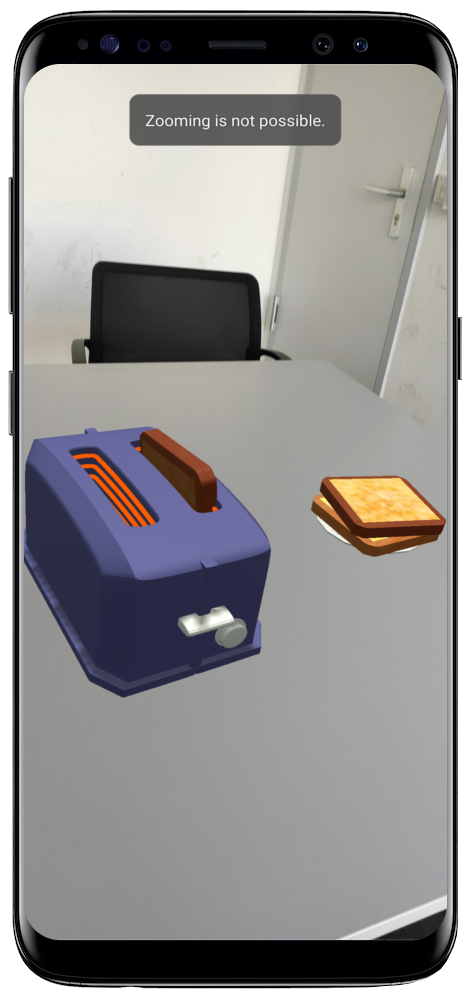
\includegraphics[width=.32\textwidth]{img/phone/phonepz1.png}
			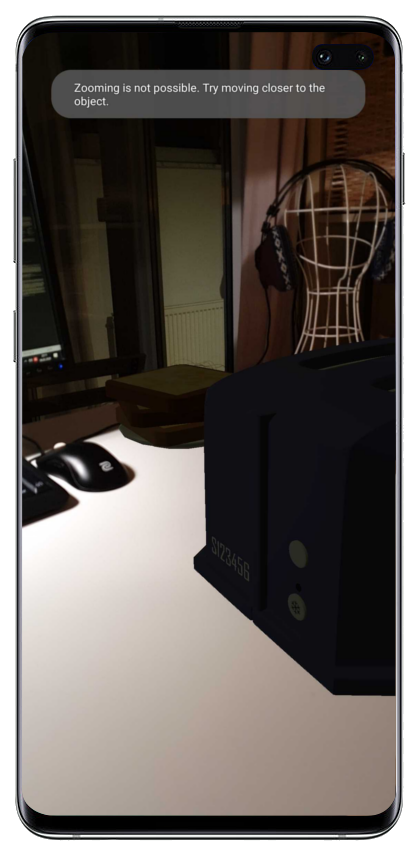
\includegraphics[width=.32\textwidth]{img/phone/phonepz2.png}
			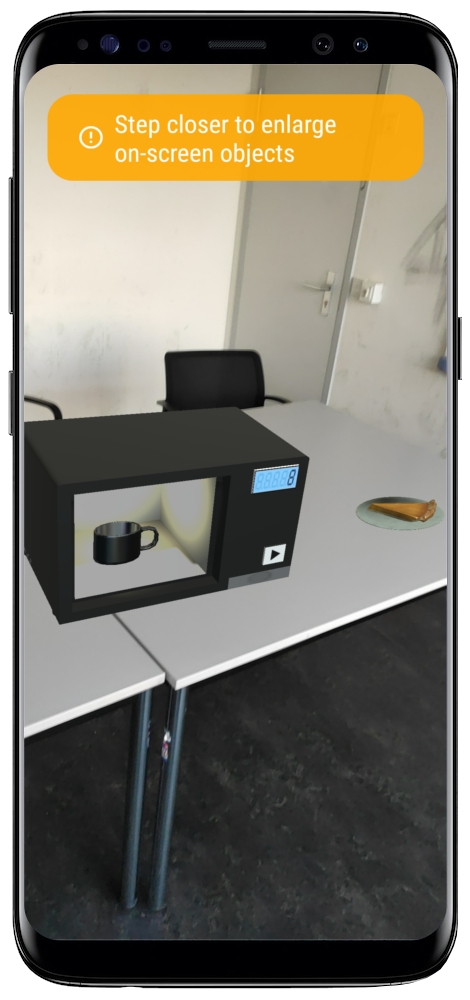
\includegraphics[width=.32\textwidth]{img/phone/phonepz3.png}
			\begin{subfigure}[t]{.32\textwidth}\centering
				\textbf{(A)}
			\end{subfigure}
			\begin{subfigure}[t]{.32\textwidth}\centering
				\textbf{(B)}
			\end{subfigure}
			\begin{subfigure}[t]{.32\textwidth}\centering
				\textbf{(C)}
			\end{subfigure}
			\caption{Three screenshots of an app made with the Vivian framework}
			\label{fig:feedbackonphone}
		\end{figure}

		% * Which frameworks/technologies were used?
		% 	* Brief info about Vivian (which relies on state machines)
		% 		* What gestures are "correct"? (vivian relies on 1 finger shit and moving environment)
		A virtual prototype is a \textit{``\textnormal{[…]} computer simulation of a physical product that can be presented, analyzed, and tested from concerned product life-cycle aspects such as design/engineering, manufacturing, service, and recycling as if on a real physical model.''} \cite{Wang2002}. The Vivian framework is an extension for Unity3D, that can be used to create mobile \ac{AR} implementations of prototypes using a 3D model and one or more finite-state machines. (sauce?)

		In a mobile app made with the Vivian framework, all user input relies on one finger gestures on the touch screen. In the example in Figure \ref{fig:feedbackonphone} (A and B) we can observe a 3D model of a toaster projected onto a live video of a real world scenario using Vivian. The user can interact with the different 3D models on the screen. Buttons can be pressed by simply tapping the screen where the respective button is displayed. Knobs and levers can be moved by putting a finger on the screen where the knob or lever is displayed, moving the finger on the screen until finding the desired position, and removing the finger from the screen afterwards. We refer to this gesture as \emph{drag-and-drop}. The Vivian framework makes a clear distinction between movable and non-movable objects in a scene. The slice of bread in the aforementioned example is movable, whereas the toaster itself cannot be moved. Movable objects can be moved in the same fashion as a lever. To cover greater distances, one can move the device itself while dragging the object. Rotation similarly requires the user to hold their finger on the object and rotate the device until they find the desired orientation. The limit of one-finger-interactions exists due to the peculiarity of \ac{AR} environments where two-finger-interactions (like a pinch-zoom or a two-finger-rotation) would be contradicting with the intended design of such an environment. If one wants to take a closer look at the previously mentioned toaster for example, they would need to step closer to the toaster.
		% * What is Usability(-testing)?
		% 	* Explain SUS (how did we tailor it to serve our purposes?)

		To evaluate different types of feedback, we decided to use usability testing as a tool to quantify the corresponding results. According to Nielsen, \textit{``usability is a quality attribute that assesses how easy user interfaces are to use. The word `usability' also refers to methods for improving ease-of-use during the design process.''} \cite{Nielsen2012}. While usability testing refers to a \textit{``observational methodology to uncover problems and opportunities in designs''} with the goal to identify problems in the design of the product or service, uncover opportunities to improve and learn about the target user's behavior and preferences \cite{Moran2019}. Therefore we chose to have the users fill out a \ac{SUS} questionnaire which we tailored to fit our needs. The basic \ac{SUS} consists of ten questions regarding a systems usability. We added a few questions which target the feedback more as well as an open feedback item, where the participants were able to share their thoughts on the system with us. 
		% graphics:
		% * all feedback message types in response to one gesture (i.e. pinch-zoom) for all prototypes, i.e.
		%	* toaster front view type 1 "pinch-zoom"
		%	* toaster rear view type 2 "pinch-zoom"
		%	* microwave front view type 3 "pinch-zoom"

	\section*{Related Work}\label{sec:relatedwork}
		% Papers (as to be found in *.bib):
		% * Dey2016: A Systematic Review of 10 Years of Augmented Reality Usability Studies: 2005 to 2014 TODO remove
		% * Nilsson2007: Fun and Usable: Augmented Reality Instructions in a Hospital Setting
		% * Poupyrev2002: Developing a Generic Augmented Reality Interface
		The topic of error handling in \ac{AR}-applications has not been broadly studied yet. There are several guidelines on how to handle wrong user input. Microsoft states in its design guidelines, that error messages should alert users of an already occurred problem. Another point they make is that the message should be suppressed if it does not make the users change their behavior or perform an action \cite{Microsoft2018}. In addition to that, Nielsen's \textit{Error Message Guidelines} demand error messages to be phrased politely. This is to avoid the implication that the user did something stupid or inherently wrong. It is also important that the messages are precise descriptions of exact problems, offering constructive advice on how to fix the problem \cite{Nielsen2001}. A 2002 IEEE article discusses two approaches of how user help might be implemented in \ac{AR} environments. What they did was to offer an icon which the users might activate themselves when they seek advice for a given task. The other feature was an automated help message that pops up when the user moves an object associated to a certain task closer to his face and tilts it. They state, that \textit{``\textnormal{[t]}his approach is more suitable for AR interfaces than traditional desktop help systems, which either distract users with a constant barrage of help messages or interrupt their work by making them search explicitly for help.''} \cite{Poupyrev2002}.

	\section*{Approach}\label{sec:approach}
		% What are "wrong" inputs? Which ones are "wrong"?
		% Describe feedback messages (size, color, content, duration) for each implementation <- graphics
		% Why these messages?
		% maybe a nice reference table for that too
		To make users quickly and easily understand the controls of mobile \ac{AR} apps, we extended the Vivian framework to provide three feedback message implementations. Each implementation's messages differ in content, colors and size (see Figure \ref{fig:feedbackonphone}). In this section, we will first describe the most common non-functional user input gestures made on the touch screen (as opposed to the gestures that were described in \nameref{sec:foundations}). Next, we present the exact content of each feedback message and the conditions under which they appear for each set of messages.

		\subsection*{Common Misconceptions in Mobile \ac{AR} User Input}\label{ssec:incorrectinput}
		In order to find feedback in response to incorrect usage of a mobile \ac{AR} application, we have to define what kinds of gestures we consider incorrect in the first place. The user interface provided by the Vivian framework is based on one finger inputs (see \nameref{sec:foundations}), therefore we should take into consideration each input that is not done with a single finger. Prominent examples for multiple finger gestures are the \emph{pinch-zoom} and the \emph{two-finger rotation}. The pinch-zoom is a gesture in which two fingers are placed on the touch screen and moved apart in opposite directions. The two-finger rotation is a gesture in which two fingers are placed on the touch screen and are together moved clockwise or counterclockwise around the center of the positions of the fingers. A two-finger rotation can also be executed by only moving one of the fingers clockwise or counterclockwise around the other finger. Common misconceptions by inexperienced mobile \ac{AR} users might include using said pinch-zoom to either zoom in on objects or to bring them closer, or using two-finger rotation to rotate objects.

		\subsection*{Feedback Message Implementations}\label{ssec:feedbackmsgs}
		The content of the first feedback message implementation is a \emph{critique}. If the user inputs a gesture that we consider incorrect, the app outputs a message that said input is not possible. For example, if a user tried pinch-zooming, they would receive a message saying: ``Zooming is not possible'' (see Figure \ref{fig:feedbackonphone}, A). The content of the second feedback message implementation is \emph{critique} and \emph{support}. We therefore refer to this feedback type as \emph{combined} in the course of this paper. The user is provided with a message stating that above mentioned input is not possible and given a hint on what they should try instead. In the scope of the previous example, such a message would say: ``Zooming is not possible. Try moving around the object'' (see Figure \ref{fig:feedbackonphone}, B). In the first two implementations, the messages have the same size and color scheme. The third implementation is more concise \emph{support}. For our previous example the exact message is saying: ``Step closer to enlarge on-screen objects''. It also differs in color scheme and size (see Figure \ref{fig:feedbackonphone}, C). Each feedback message in every implementation is displayed for 5 seconds.

		\begin{center}
			\begin{tabular}{|C{.05\textwidth}|L{.15\textwidth}|L{.23\textwidth}|L{.45\textwidth}|} \hline
										& \textbf{Description}												& \textbf{Gesture (input)} 					& \textbf{Response (output)} 											\\ \hline
				\multirow{2}{*}{\#1}	& \multirow{2}{*}{\parbox{.15\textwidth}{critique}}					& two-finger rotation						& Rotating the object is not possible.									\\ \cline{3-4}
										& 																	& pinch-zoom								& Zooming is not possible. 												\\ \hline
				\multirow{2}{*}{\#2}	& \multirow{2}{*}{\parbox{.15\textwidth}{combined}}					& two-finger rotation						& Rotating the object is not possible. Try moving around the object.	\\ \cline{3-4}
										& 																	& pinch-zoom								& Zooming is not possible. Try moving closer to the object.				\\ \hline
				\multirow{3}{*}{\#3}	& \multirow{3}{*}{\parbox{.15\textwidth}{support}}					& two-finger rotation (movable object)		& Hold the object and move the phone to rotate							\\ \cline{3-4}
										& 																	& two-finger rotation (elsewhere)			& Move around the objects												\\ \cline{3-4}
										&																	& pinch-zoom 								& Step closer to enlarge on-screen objects								\\ \hline
			\end{tabular}
			\captionof{table}{The responses for each input in each implementation.}
			\label{tab:feedback}
		\end{center}

		The contents of each message can be found in Table \ref{tab:feedback}. The description column holds the names we assigned to the three different feedback implementations. In the gesture and response columns you can find the corresponding inputs and outputs respectively. If for example a user tried a two-finger rotation in the critique implementation, the app would display a message saying ``Rotating the object is not possible''.
		In the support implementation we made the distinction between two-finger rotations on movable objects and elsewhere. If the aforementioned center point of the two-finger rotation is placed on a movable object (see \nameref{sec:foundations}), the app displays the message that corresponds to ``two-finger rotation (movable object)''. If the two-finger rotation is executed elsewhere, the ``two-finger rotation (elsewhere)'' message is displayed instead.
		We recognize user input using a software library called TouchKit. TouchKit provides an easy way to detect gestures such as our two-finger rotations and pinch-zooms. For two-finger rotations, we set a tiny minimum angle threshold. If the two-finger rotation's angle is smaller than this threshold, it is ignored and no message is provided. Likewise for pinch-zoom, we set a minimum distance threshold.
		To further ensure clear distinction of the gestures, we disable the pinch-zoom recognition while two-finger rotation is currently recognized and vice versa.


	\section*{Case Study}\label{sec:casestudy}
		%unfixed:
		%- why in the domain of usability engineering?
		%- mentioned Vivian Framework, where should it be exactly?
		%- time tenses
		%- all p-values should be given (statistics)
		
		To evaluate the quality of our feedback implementations we conducted a case study in the domain of usability engineering, which is presented in this section. In the section ``\nameref{ssec:setup}'', we describe in detail what each participant in the case study had to do and what data we collected. The results of the study are found in \nameref{ssec:results} and afterwards discussed in \nameref{ssec:discussion}.
		
		\subsection*{Setup of the Case Study}\label{ssec:setup}
			In order to evaluate, which variant in our approach works best, we created two different prototypes with the Vivian framework (see \nameref{sec:foundations}). Both of them are quite simple kitchen devices: a toaster prototype and a microwave prototype (as seen in Figure \ref{fig:feedbackonphone}).

			The microwave's functionality is limited to heating an object inside it with constant power. Figure \ref{fig:feedbackonphone} C shows this prototype in an application. It has one button to add 10 seconds to the heating duration and another one below to open the door. The door can be closed by moving it. The status of the microwave is visually indicated by a small display showing the remaining heating time or ``ready'' in idle mode and a light inside the device, which turns on when it is heating or when the door is opened. A serial number is printed on the back of the microwave. The prototype scene is completed by two additional objects. A cup that is already in the microwave when the application launches and a piece of cake on a plate next to it. These objects are moveable by the user.

			The toaster can toast one or two pieces of bread at a time. Figure \ref{fig:feedbackonphone} A shows the front of the prototype in an application and figure \ref{fig:feedbackonphone} B its back. The toasting can be started by pulling down a lever at the front and stopped by pushing it up again or by pressing the stop button, which is on the back. Otherwise, the toasting stops automatically after a time which is defined by the position of a rotatable knob at the front. The time mode is divided into low, medium and high duration. Further functionality is provided by the unfreezing mode, which can be activated using the snowflake button on the back. The activation of the unfreezing mode results in a longer toasting duration and is indicated by a light above the button. The toasting process itself is displayed by the glowing of the heating elements, which is visible in figure \ref{fig:feedbackonphone}-A. The toaster prototype also has a serial number on its back. The prototype scene is completed by a stack of 3 pieces of bread lying next to it. 
			
			Based on these functionalities we designed three tasks per prototype, which are shown in Table \ref{tab:tasks}. The tasks are increasing in complexity. An example of this increase is that in task 2 of the microwave we ask to heat the cup, which is already in the microwave, for any amount of time. Therefore, only the start button has to be pressed once to fulfill this task. Afterwards, in task 3, we ask to replace the cup with the pie and heat for a specific amount of time. This task contains more necessary steps: opening the door, moving the cup out, moving the pie in, closing the door, pressing the start button multiple times and finally pressing the stop button after the desired amount of time.

			\begin{center}
				\begin{tabular}{|C{.05\textwidth}|L{.41\textwidth}|L{.41\textwidth}|}
					\hline \textbf{\#} & \textbf{Microwave} & \textbf{Toaster} \\
					\hline 1 & Read serial number of the microwave & Read serial number of the toaster \\
					\hline 2 & Heat up the cup & Toast the bread \\
					\hline 3 & Remove the cup, put the pie in, set the timer to 20 seconds and remove the plate at 5 seconds & Toast the bread on high heat and put the toaster in unfreezing mode \\
					\hline
				\end{tabular}
				\captionof{table}{The tasks for the different prototypes.}
				\label{tab:tasks}
			\end{center}

			For the case study, we divided the participants into four groups. Each of these groups tested one version of the app on a mobile phone. The versions differed in the feedback given (see \nameref{sec:approach}). We gave no feedback at all to the participants in group 0, which is our control group. Participants in group 1 got our first implementation with \emph{critique} feedback. In group 2 they got our second implementation with a \emph{combined} feedback version and in group 3 they got our third implementation with \emph{supportive} feedback (see Table \ref{tab:feedback}). Each participant was asked to fulfill the tasks for each prototype in the order provided in Table \ref{tab:tasks}. One half of the participants were asked to do the tasks of the toaster prototype first, while the other half did the tasks for the microwave prototype first. This divide was equally for all groups. We were able to evaluate subgroups with a certain implementation level and a certain order of prototypes they tested. In the following, the subgroups are named \emph{TM}, which translates to ``first toaster, then microwave'' and \emph{MT}, which translates to ``first microwave then toaster'', followed by the number of their feedback group. For example, a participant who was assigned the toaster first and then the microwave without any feedback was in the subgroup TM0.

			Before the start of the test, we gave every participant a short introduction. This introduction contains information about the mobile \ac{AR} technology and reasons behind usability testing to prepare the participants and create a similar level of expectation. It deliberately does not contain information about how to use the application or the scope of the case study. This is important so the participants are not biased about wrong usage and the feedback they would get. During the test, we used screen recordings to measure each participants' use of the application. These enabled us to acquire completion times for the different tasks and count the number of incorrect usages. We used a notepad to register further observations.

			Following the test of the application, the participants were asked to fill in a questionnaire. This questionnaire consists of 3 parts. First we asked participants if they had used \ac{AR} applications before. The second part is an \ac{SUS} (see \nameref{sec:foundations}) about the usability of the \ac{AR} application, that we tailored for our needs. The third part is an open question directly aimed to the feedback provided by the application, namely: \emph{``If you have any suggestions on what kind of feedback from the app you would find better, please let us know''}.

		\subsection*{Results of the Case Study}\label{ssec:results}

			We conducted the case study with 10 participants per feedback group. This leads to 40 people participating in the case study in total. The smallest subgroups, defined by implementation and task order, were still filled with 5 participants. 21 of the 40 participants said they had prior experience with \ac{AR} applications. The group with the highest prior knowledge was the control group with 7 of 10 participants. The groups for the \emph{critique} feedback and the \emph{combined} feedback both had 6 participants with prior knowledge, while the group with the \emph{support} feedback had just 2 participants, who said they had prior knowledge.

			In our approach, we consider especially two gestures as incorrect usage: the pinch-zoom and the two finger rotation (see \nameref{sec:approach}). With the setup of our case study, the two finger rotation appeared more often than the pinch-zoom gesture. Figure \ref{fig:tfr_v_pz} shows the appearances of two finger rotations and pinch-zooms for all tasks given to the participants in the case study. In total over all participants and all tasks, two finger rotations appeared 225 times, while pinch-zoom appeared 51 times. Since 82\% of the incorrect usages are two finger rotations, the results of our case study focus on those. We especially evaluate the second task for the toaster, since it was most demanding for the users. As shown in Figure \ref{fig:tfr_v_pz} A, 91\% of the overall two finger rotations occurred in that task. Also the majority of pinch-zoom gestures occurred there.

			\begin{figure}[H]
				\centering
				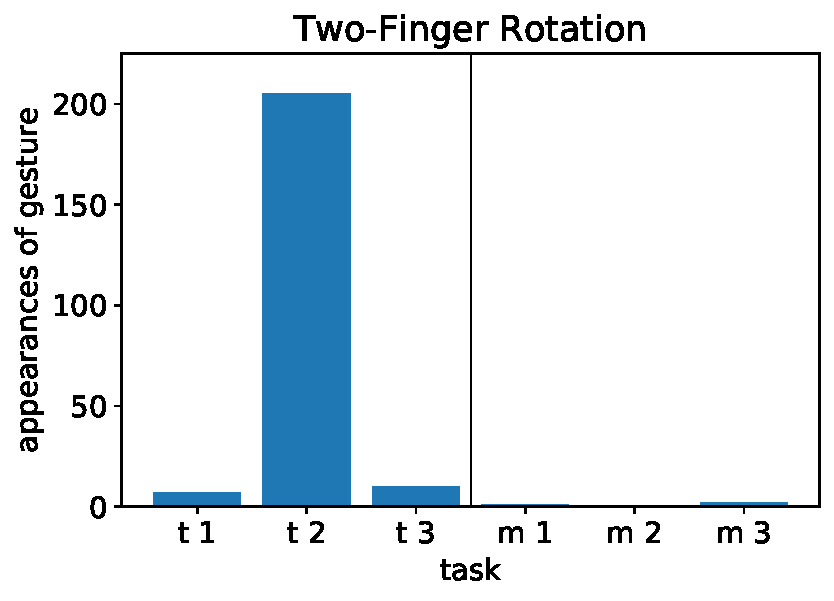
\includegraphics[width=.49\textwidth]{img/plot/plot_tfr.pdf}
				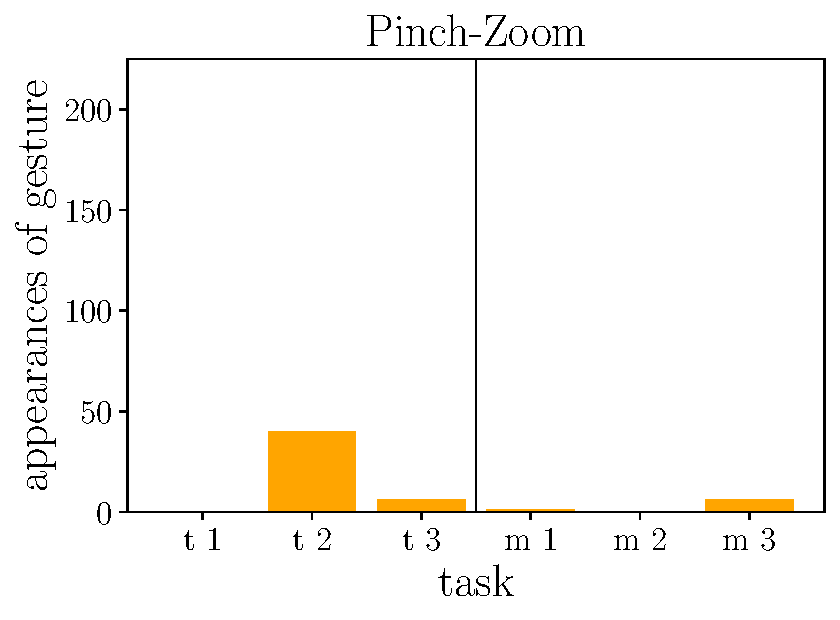
\includegraphics[width=.49\textwidth]{img/plot/plot_pz.pdf}
				\begin{subfigure}[t]{.49\textwidth}\centering
					\textbf{(A)}
				\end{subfigure}
				\begin{subfigure}[t]{.49\textwidth}\centering
					\textbf{(B)}
				\end{subfigure}
				\caption{Appearances of the two finger rotation gesture and the pinch-zoom gesture per task of the case study. }
				\label{fig:tfr_v_pz}
			\end{figure}

			To evaluate the effectiveness of the different implementations, we compare the users' behavior for the second task of the toaster, with different measures. Figure \ref{fig:t2_metrics} shows box plots for the two most important measures. The diagram in Figure \ref{fig:t2_metrics} A gives the time participants needed to fulfill the task by their case study group. The median is given by the line inside the box. The box itself gives the 25 percentile on its lower bound and the 75 percentile on its upper bound. The whiskers are defined by the last data points which are within the range of 1.5 times the IQR. For clarification the data points are printed semi-transparent over the box plot. Figure \ref{fig:t2_metrics} B is similar: it shows the two finger rotation attempts per user for the different case study groups. Important for this graph is that users, who had zero two finger rotation attempts, are excluded from the statistic. The reason behind it is that these users didn't receive any feedback message independently of their given implementation. To trigger any feedback, an incorrect usage must occur at least once. In total, 4 of the 40 participants didn't try any two finger rotations on this task. The maximum number for one specific implementation is 2. That means that for each implementation at least 8 participants' data was used to take the statistical values.

			\begin{figure}[H]
				\centering
				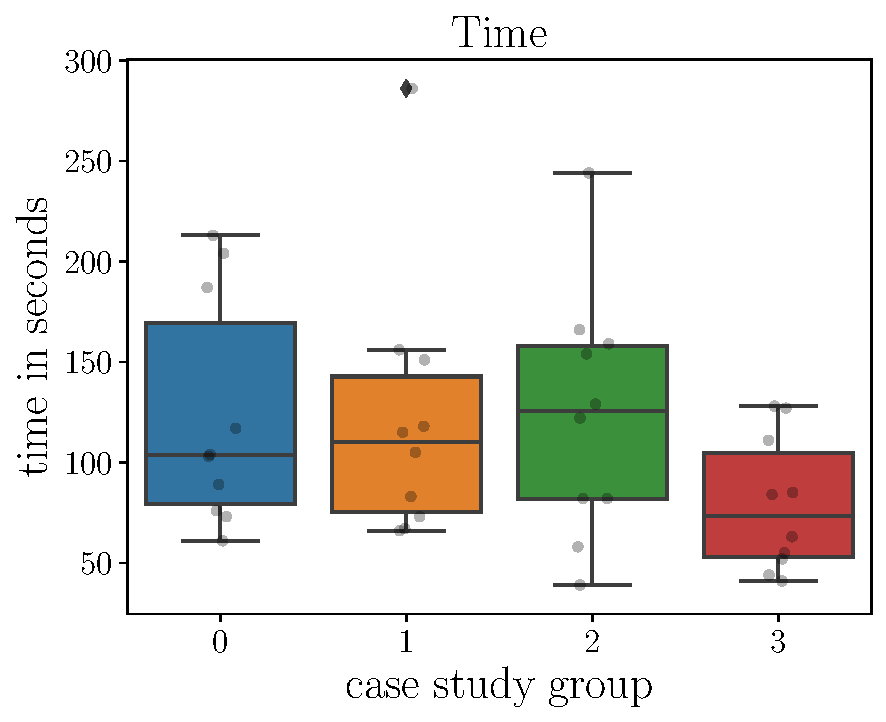
\includegraphics[width=.49\textwidth]{img/plot/plot_bplot_time.pdf}
				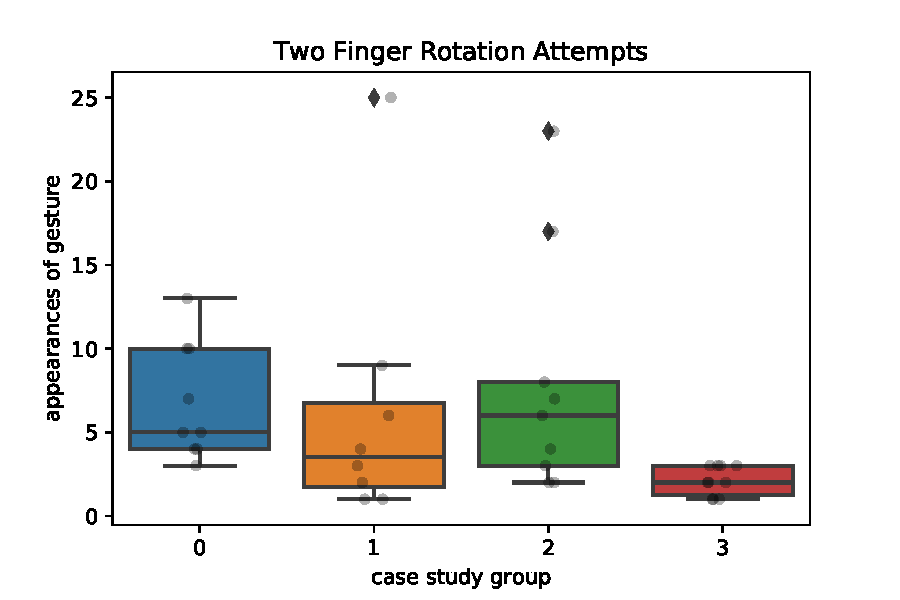
\includegraphics[width=.49\textwidth]{img/plot/plot_bplot_tfr.pdf}
				\begin{subfigure}[t]{.49\textwidth}\centering
					\textbf{(A)}
				\end{subfigure}
				\begin{subfigure}[t]{.49\textwidth}\centering
					\textbf{(B)}
				\end{subfigure}
				\caption{Evaluation of the two finger rotation attempts and time needed for the 2nd task for the toaster prototype.}
				\label{fig:t2_metrics}
			\end{figure}

			To check whether the result is statistically significant, we performed statistical tests on both the time needed to complete the task and the number of two finger rotation attempts. The main test is the \emph{Welch t-test}, that is used to compare the different implementations with the control group, which didn't receive any kind of feedback messages. The \emph{Welch t-test} has the assumption that both populations are normally distributed. We used the \emph{Shapiro-Wilk} test on the residuals between the given implementation group and the zero feedback group to check on the assumption. Generally we consider p-values below 0.05 as statistically significant. Table \ref{tab:pvalues} shows the p-values for the different tests for all three implementations. The \emph{Shapiro-Wilk} tests does not indicate normality for the two finger rotation metric with the \emph{critique} feedback implementation and the time metric with the \emph{combined} feedback implementation. Since the assumption for the \emph{Welch t-test} is not given, the test cannot be run for these two cases. In all other cases the assumption that the data is normally distributed holds. For the \emph{critique} and the \emph{combined} feedback implementations the test with the other metric did not reveal any significant difference to the control group. For the \emph{support} feedback implementation the result of the \emph{Welch t-test} for the number of two finger rotation attempts in task 2 of the toaster prototype implies a significant difference to the control group, which however cannot be fully confirmed by our result for the completion times for the task.

			\begin{center}
				\begin{tabular}{|L{.22\textwidth}|L{.22\textwidth}|C{.22\textwidth}|C{.22\textwidth}|} \hline
					\textbf{statistical test}		& \textbf{implementation}	& \textbf{p-values: two finger rotation} 		& \textbf{p-values: time} 											\\ \hline
					\multirow{3}{*}{Shapiro-Wilk}	& critique					& 0.001							& 0.972								\\ \cline{2-4}
													& combined					& 0.420							& 0.029 								\\ \cline{2-4}
													& support					& 0.971							& 0.507								\\ \hline
					\multirow{3}{*}{Welch t-test}	& critique					& -								& 0.980								\\ \cline{2-4}
													& combined					& 0.681							& -									\\ \cline{2-4}
													& support					& 0.010							& 0.054 									\\ \hline
				\end{tabular}
				\captionof{table}{p-values of statistical tests for the time needed to fulfill the 2nd task for the toaster prototype and the two finger rotation attempts in that task.}
				\label{tab:pvalues}
			\end{center}

			In addition, we evaluated the relationship between our two metrics for the task. The correlation coefficient between the time and the attempts of two finger rotation is 0.43, which indicates a moderate positive relationship between the metrics. Figure \ref{fig:scatter} visualizes the relationship between the time needed for the task and the number of two finger rotation tries. The color of a data point is set by the implementation used by this participant. One can observe that the participants with implementation 3 are all clustered with a low time and a low amount of two finger rotations, while all other groups are more randomly spread.

			\begin{figure}[H]
				\centering
				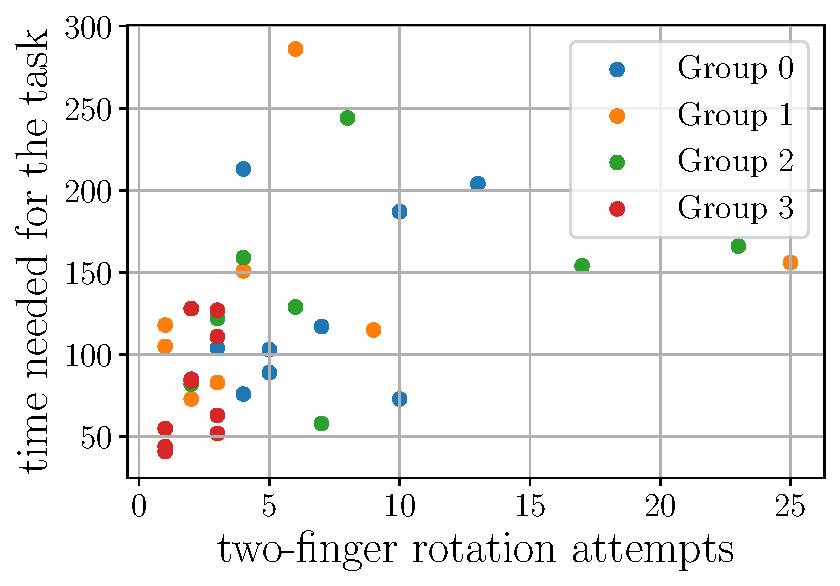
\includegraphics[width=.49\textwidth]{img/plot/plot_scatter.pdf}
				\caption{DUMMY: Time needed to fulfill the 2nd task for the toaster prototype depended on the number of tfr tries.}
				\label{fig:scatter}
			\end{figure}

			For the evaluation of the questionnaire, we calculated the \ac{SUS} scores for every participant. Figure \ref{fig:sus} shows the scores mean for each case study group. The horizontal red line is at a score of 68, which in terms of \ac{SUS} stands for average usability (see \nameref{sec:foundations}).

			\begin{figure}[H]
				\centering
				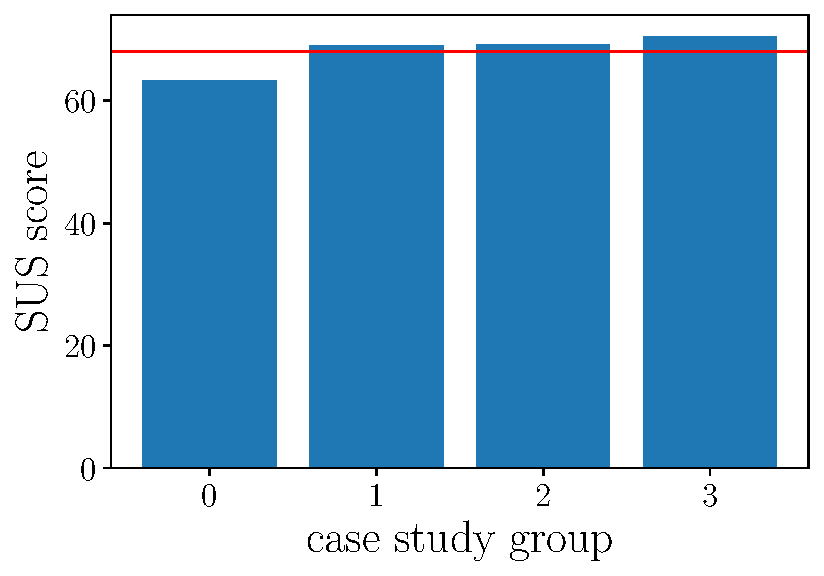
\includegraphics[width=.49\textwidth]{img/plot/plot_sus.pdf}
				\caption{SUS score by the case study groups.}
				\label{fig:sus}
			\end{figure}

			24 of the 40 participants answered the open question (\emph{``If you have any suggestions on what kind of feedback from the app you would find better, please let us know''}). We categorize the answers with four different labels, divided by the topic the answer is about. These are \emph{app feedback}, \emph{app controls}, \emph{prototype design} and \emph{other}. Answers in the \emph{app feedback} category are directed to the provided feedback messages or other desired feedback. Answers in the \emph{app controls} category are about struggles with or improvement ideas for the applications controls. The \emph{prototype} category is related to the prototype design and its usability, for example button sizes. The last category, \emph{other}, is summing up single appearing answers which scope is not relevant for this research. The appearances of the different types of answers are listed in Figure \ref{fig:tags}. In case an answer fit to multiple labels, we count it for all the fitting categories.

			\begin{figure}[H]
				\centering
				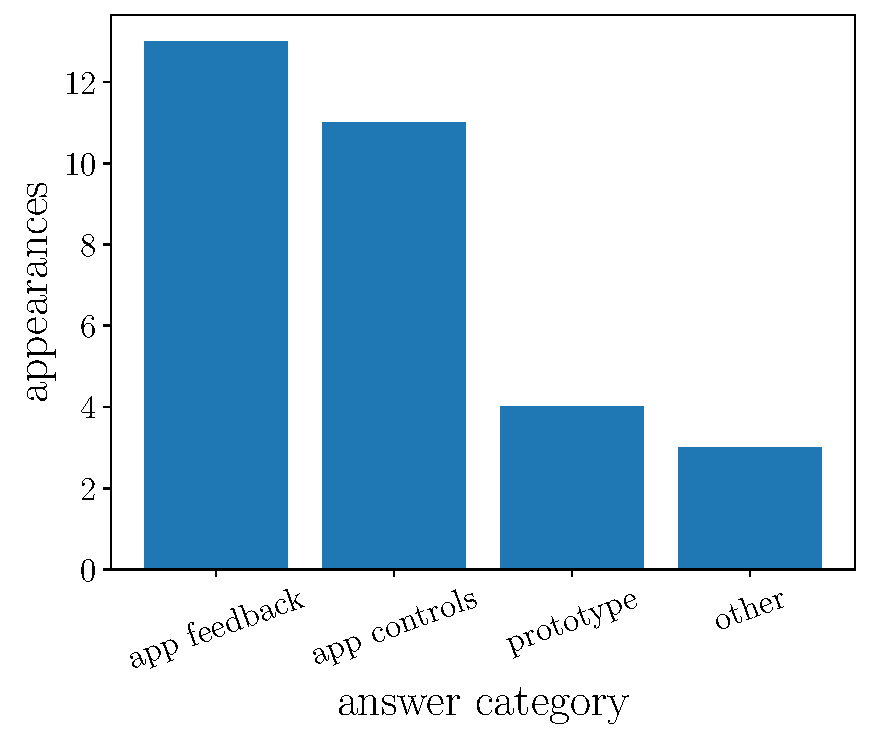
\includegraphics[width=.49\textwidth]{img/plot/plot_tags.pdf}
				\caption{Categorized open question answers.}
				\label{fig:tags}
			\end{figure}
			
			For a deeper evaluation of the answers we split them by the case study groups (see Figure \ref{fig:tags_imp}). 
			Most of the answers related to \emph{app feedback} came from participants in the control group. All of this answers were asking for any kind of help. A lot directly asked for text messages providing help. Also the ideas of a help button or an introduction, which explains the controls were mentioned. Participants in the other groups also mentioned additional help implementation methods, like vibration feedback or help for the specific task from the application. Answers directed to our feedback message implementations were that they could be hidden by the fingers, when the user turns the phone and a participant with the \emph{combined} feedback mentioned that the message should be visible for a longer duration. The other big category of the participants' answers is \emph{app control} related. They have in common that the rotation of the piece of bread in the second task for the toaster prototype was not easy to archive for them. Also some were mentioning that the two finger rotation could be the more intuitive option.

			\begin{figure}[H]
				\centering
				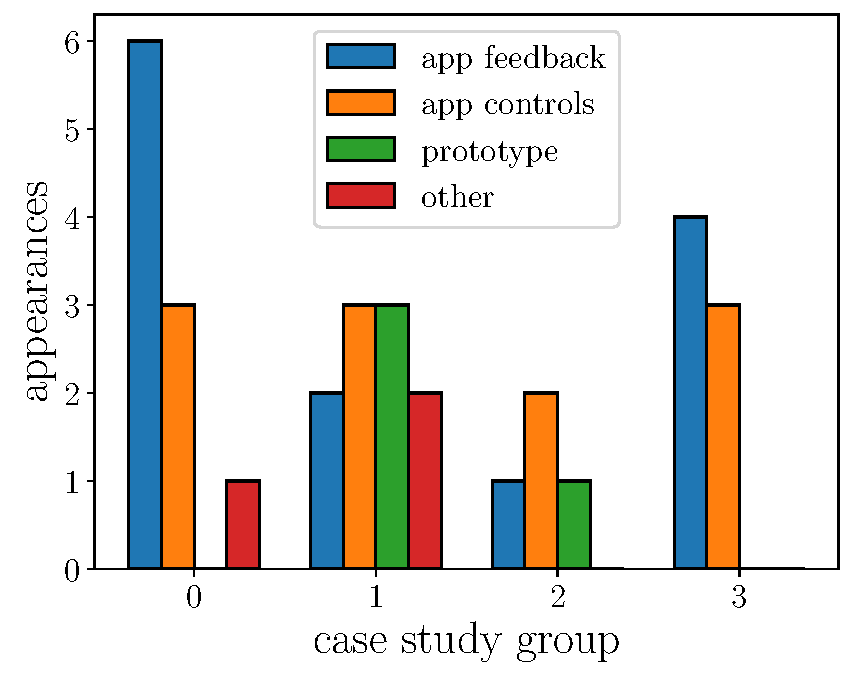
\includegraphics[width=.49\textwidth]{img/plot/plot_tags_implementations.pdf}
				\caption{Appearances of answer categories by the participants case study groups.}
				\label{fig:tags_imp}
			\end{figure}


		\subsection*{Discussion of the Case Study Results}\label{ssec:discussion}
			% discussion of the results in the previous section
			% "threats to validity" part
				% DISCUSSION
		% * hypothesis "visible and better feedback msg help the user to fulfill tasks faster, easier"
		% * feedback message must be genera enough to be applicable to any possible situation
		% * feedback message must be specific enough to be more helpful in the given situation
		% * outlines: sus/free answers
		% * easy prototype microwave -> intuitively usable, no feedback needed
		%
		% THREATS TO VALIDTY
		%
			With the given setup of our case study the two finger rotation gesture appeared more often than the pinch-zoom gesture (see figure \ref{fig:tfr_v_pz}). Usually, users attempt the pinch-zoom gesture when an object on the screen is too small to see or use. Our participants started right in front of the object, so there was no need to step much closer to it. Also, for simplicity's sake, the prototypes were not created with unnecessarily small controls, which means all of them were well visible in general. Clearly, there are other applications where users are more tempted to use this gesture. It is likely that outcomes of the evaluation of feedback messages for incorrect usages for rotation are applicable in a similar way for zoom and other functionalities. We have to divide the evaluation of the rotation into two groups, as we do for our \emph{supportive} feedback implementation (see \nameref{sec:approach}). While most of the users intuitively walked around objects to rotate their view on the scene, they struggled more with rotating a certain object, namely a piece of bread in this case. This is the reason why the second task for the toaster prototype is most important. The specific task is just ``Toast the bread'', but this includes rotating the object laying on the plate (see \ref{fig:feedbackonphone} A) by $90\degree$ to put it into the device. The struggle with this task also becomes visible by the fact that only 10\% of the participants were able to do it intuitively without trying a two finger rotation before. Therefore most users could profit from helpful feedback.

			The feedback versions we provided performed differently in the case study. While the implementation with \emph{critique} feedback and the implementation with \emph{combined} feedback did not had a significant effect, the users with the \emph{support} feedback were able to fulfill the task in less time and with significantly less attempts of the incorrect two finger rotation gestures. Prior knowledge about the usage of \ac{AR} applications can not be a reason for it, because this groups participants had the lowest percentage of prior knowledge. Instead we can assume multiple reasons for this difference. One is that the \emph{support} feedback implementation has a better visibility than the other two (see \ref{fig:feedbackonphone}). While the other two implementations provide messages looking like the typical Android pop-up messages, the \emph{support} feedback messages are larger and have a orange color instead of gray. Additional the messages of this implementation are shown for a longer duration. All this changes are there to make the messages more eye-catching for the users. This matches with our observation during the test that some of the participants with the \emph{critique} or \emph{combined} ignored the messages, which did not happen for participants with the \emph{support} feedback. The other difference is the helpfulness of the messages' content. The \emph{critique} feedback just tells the users what they have done incorrect, but not how they do it correctly. Since the actual rotation gesture was not intuitive for most participants, they could not come up with the right idea for rotation easily themselves. Our \emph{combined} feedback implementation has a similar issue. The message popping for any kind of rotation is \emph{``Rotating the object is not possible. Try moving around the object.''}. This message does not provide the right help for the most challenging task, which is the rotation of the piece of bread, because it is designed for the wrong kind of rotation. The \emph{support} feedback message serves better with \emph{``Hold the object and move the phone to rotate''}, because its specific enough to help in the given situation.			
			
			Our data states that participants perform significantly better with the \emph{support} feedback implementation, but we also asked the participants to assess their experience with our \ac{AR} application themselves. Figure \ref{fig:sus} shows that the average \ac{SUS} result of participants in case study group 3 with the \emph{support} implementation is only slightly higher then the others. So the impact on how the participants feel the usability is not as strong as the impact on how they actually perform. We asked the participants to assess the usability of the overall AR application, since that is what the feedback messages should serve to. Unfortunately other aspects have an impact on the general experience too. Also the users strongly rated the usability of the prototype itself, because we tested the usability of our feedback with the use of the prototypes. That is why our case study groups are too small to evaluate the \ac{SUS} results. The answers to the open question fit to this impression. We asked them to give us opinions directly on the feedback the application provided or did not provide, in case of the control group. Still almost as many participants reacted to the app usage (\emph{app controls}) as to the \emph{app feedback} as shown in Figure \ref{fig:tags}.
			


			%Ideas for Outlook (not ordered):
			% like implementation 3 is good
			% visibility v helpfulness
			% What was the reason? better visibility or better content?
			% another case study for other wrong usages.
			% Hand in front of camera issue
			% introduction instead? 
			% more intuitive rotation implementation?


	\section*{Summary and Outlook}\label{sec:summary}
		This paper aims at contributing towards improving the overall mobile \ac{AR} experience of users by providing them the appropriate feedback in case of usage of unsupported gestures. We developed three different sets of feedback messages and conducted a case study to test different tasks with users which were divided into four different groups. Users in different groups received different types of feedback messages. The feedback messages were implemented as an extension to a mobile \ac{AR} framework called Vivian. The \nameref{sec:approach} and \nameref{sec:casestudy} sections describe in detail the feedback types and how users were divided into different groups.
		
		In our work, we focused on the pinch-zoom and the two-finger rotation, which are incorrect input gestures described in \nameref{ssec:incorrectinput} and therefore not supported by Vivian. According to our findings, users are inclined to use two-finger rotations when they are confronted with a task in which they have to rotate an object in order to complete it. Our results support that appropriate feedback does indeed help users complete such tasks in less time. In our case study, users with appropriate, supportive feedback were completing the first rotation task twice as fast as users without any feedback. Moreover, during the completion of tasks, the number of incorrect gestures for each user with appropriate feedback was three to four times smaller in comparison to the number of incorrect gestures for each user without feedback. Pinch-zoom gestures however were not widely used by our participants, which is most likely due to our test setup (see \nameref{ssec:discussion}). The feedback type that we found most effective among the ones we implemented in the course of our case study is the supportive one. The exact content of the messages can be reviewed in \nameref{ssec:feedbackmsgs}. The messages in that implementation are not only more accurate, they are also provided with the brightest colors and biggest font.

		Pinch-zoom gestures are not yet taken into account by our case study setup, which makes it impossible to evaluate the feedback implementation we developed in the scope of this gesture. Further we noticed <X> of our 40 participants were trying to interact with on-screen objects by moving their hand in front of the camera lens of the mobile device instead of using the built-in touch screen. Since our results look promising, we will conduct another case study in the future, where we consider these observations in the case study setup. We will also consider other feedback types with different visibility and content, to discover whether the effect we found is due to one or another.

	\pagebreak
	\printbibliography
\restoregeometry
\end{document}